\documentclass[19pt]{article}

\usepackage{arxiv}
\usepackage{makeidx}
\usepackage{fancyhdr}

\usepackage[utf8]{inputenc} % allow utf-8 input
\usepackage[T1]{fontenc}    % use 8-bit T1 fonts
\usepackage{hyperref}       % hyperlinks
\usepackage{url}            % simple URL typesetting
\usepackage{booktabs}       % professional-quality tables
\usepackage{graphicx}
\usepackage{amsfonts}       % blackboard math symbols
\usepackage{amsmath}
\usepackage{nicefrac}       % compact symbols for 1/2, etc.
\usepackage{microtype}      % microtypography
\usepackage{lipsum}

\pagestyle{fancy}
\title{AI in Medicine : Identification and Localization of Metastatic Tissues in histopathelogical scans of Lymph Nodes} 


\author{
    Spandan Ghosh\thanks{Apart from the above mentioned email address, several relevant background knowledge and information is available on \url{https://spandanji.github.io}}\\
    Department of \emph{Electronics and Communication Engineering}\\
  Institute of Engineering \& Management\\
  Kolkata, India \\
  \texttt{spandanghosh2@gmail.com} \\
}
\begin{document}

\maketitle

\begin{abstract}
    Artificial Intelligence has been setting the benchmark for almost all commercial and research fields. Since the rapidly growing popularity of these approaches now draw the interests of the people in the resepective fields of application, we now define state of the art benchmarks with respect to how well several networks perform in different fields. Medical Imaging and the analysis of these images are no different. The polished techniques in Digital Image Processing such as the various filters, transforms, thresholding techniques have already been in use to reduce redundant human work when these techniques can perform pattern recognition for trivial, repititive tasks. The effect of the evolution of Deep Learning has allowed the learning of complex convolution filters using Convolutional Neural Networks(CNNs) which now permit the detection of intricate patterns and segmenting them to such an extent that these now become more efficient than the human eye in several cases. Medical Images however, post various challenges that are usually absent in other applications of Deep Learning in Computer Vision. 

    The first and primary issue is the quantity of data available. The amount of data available is nowhere close to the other real world applications such as classification of cusines by their snapshots. Moreover, medical images cannot be readily scraped or taken from the real world. Taking the problem at hand, one cannot simply step out into the world and acquire scanned and labelled images of Lymph Tissues. Their aquisition depends on Medical Institutions. Furthermore, the process of capturing, labelling, processing and releasing such a dataset is difficult and requires specialized attention from medical professionals. The second issue is that this, combined with the fact that expensive equipment may be required for their collection makes the process expensive.

    Segmentation adds another complexity:\textbf{The complexity of effort}. Segmentation involves a pixel to pixel mapping between the input and an output. Every single tissue sample image needs to be segmented by a medical expert for us to train an algorithm to do so automatically on other images. This process is tedious. In this project, along with reviewing certain approaches of interest, I am going to achieve the a segmentation map on the input image without using a segmentation levels and am also going to discuss some alternative methods in which the above claimed can be achieved and when and where which should be preferred.
    
\keywords{Semantic Segmentation\and Medical Image Analysis \and Associative Networks \and Deep Learning}
\end{abstract}
\newpage
    \tableofcontents
\newpage
% keywords can be removed



\section{Introduction}
The upsurge in the dominance of Deep Learning in defining the Statei-of-the-Art in a great variety of fields. Both Research and Industrial organizations all over the world are on a lookout to capitalize on the edge provided by Deep Learning and to leverage an increase in performance or profit in accordance with the goals of the organization. With data being in abundance in this digital age and the greatly evolved compute capacity with the rise of GPUs (Graphical Processing Units), the tedious and compute hungry processing of training models on particular datasets has become easier and practically feasable.

\subsection{Motivation}
There has been a huge upsurge in the replacement of tedious and laborious work with algortihms to automate the process. Segmentation is no different. Segmentation is the process of reconstruction of an input image as the output image with certain pixels of the image highlighted or labelled to be of a particular class or to have a particular property. In Medical Imaging, this is quite often required in the highlighting of infected regions or affected areas in cells or scans. Before getting into the approaches in Digital Image Processing and Deep Learning to solve such problems, let us have a look at some typical segmentated images.

\begin{center}
    \begin{figure}[!h!t!b]
        \centerline{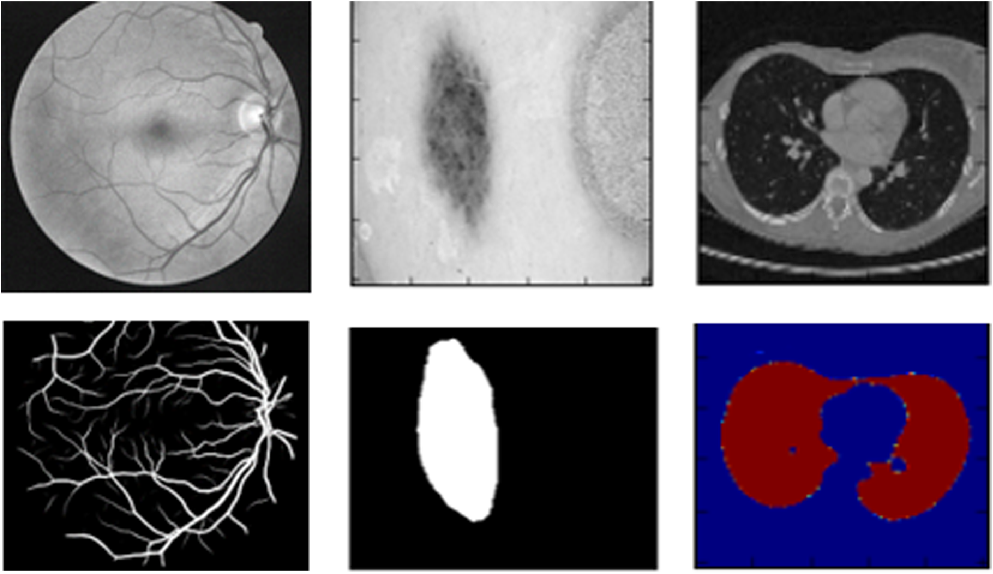
\includegraphics[width=105mm,height=65mm]{images/segs.png}}
        \caption{Some Segmented images : Row-1 has the input images and row 2 has the output images also known as the segmented images or the segmentation maps}
        \label{fig:1}
    \end{figure}
\end{center}

Segmentation is not limited to the world of medical prognosis. It is applicable in several fields of interest such as Handwriting analysis as seen in Kaur et. al.\cite{kour2014real}. The usual idea behind segmentation would be to design a mathematical function that proposes a mapping between input and output pixels. As seen in Fig. \ref{fig:1}, the left-most image is one that segments the retinal vesicles of the eye. Such a work would require constant supervision and analysis of such images manually by medical professionals as such a work requires a degree of domain knowledge and expertise.

This problem is one typical area where we would want to apply Image Processing to either independently solve the problem or to make the job easier by minimizing the human sipervision involved. The motivation as such, behind my analysis of approaches and the development of the project is the explotation of data to learn functions that map from the input image to the output image. However, such a task requires data in such a format that every input image has a corresponding output image in the dataset and this needs to be prepared as the dataset by the said professionals. 

This project shall deal with a detailed comparative analysis on several different approaches on that are used in Semantic Segmentation but also discuss the main process under consideration where we DO NOT have to use segmentation data but we can still Localize the affected areas simply from the available data. This project shall be beneficial for the localization of cells with or without segmentation data and if segmentation data is available, the comparative analysis shall help in the choice of approach as will be beneficial for the project. 

\subsection{Objective}
The Objective of this project is to achieve the localization of cancerous cells in slides containing lymph tissues in general. The specific problem we shall be dealing with is the identification of metastatic tissues in the histopathelogical scans of lymph node sections. 

\begin{center}
    \begin{figure}[!h!t!b]
        \centerline{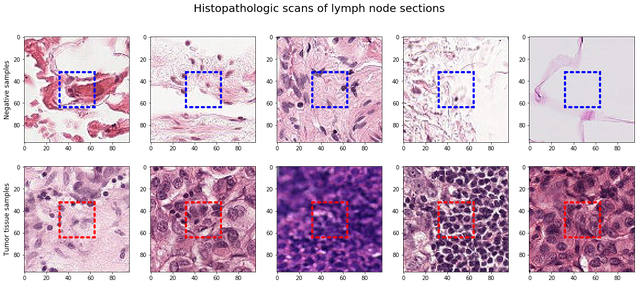
\includegraphics[width=105mm,height=65mm]{images/metastases.png}}
        \caption{The cells and a certain box showing the areas of possible interest}
        \label{fig:2}
    \end{figure}
\end{center}

\begin{center}
    \begin{figure}[!h!t!b]
        \centerline{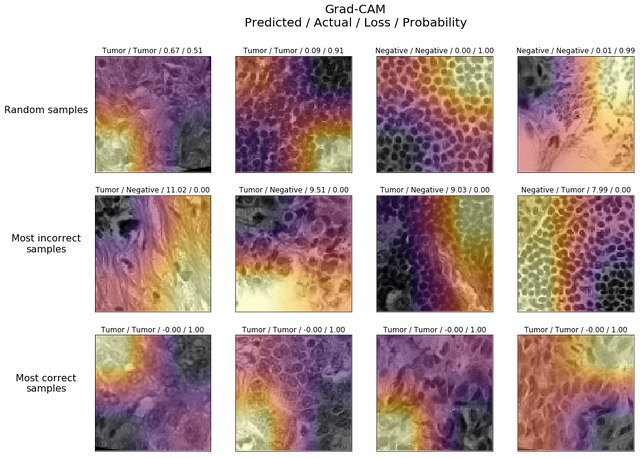
\includegraphics[width=105mm,height=65mm]{images/gradcam.png}}
        \caption{Gradcam or the regions in the input image that most affect the output in the image}
        \label{fig:3}
    \end{figure}
\end{center}

In Fig \ref{fig:2} , we the images we see are the input images. These are the histopathelogical scans of lymph node sections. The data is such that each scan is labelled healthy and unhealthy. For this dataset we do not have a segmentation map available, and yet our objective shall be to localize the areas of interest which have caused the activation to be positive or negative. In other words we shall aim to effectively superimpose heat maps as shown in Fig \ref{fig:3} such that we solve the purpose of segmentation as surely such regions of interests are the patterns corresponding to the scan being healthy or unhealthy ie. they are the cancerous or metastatic regions. 
\subsection{Organization of the Report}
    This report shall be devided into several sections. We shall first have a look at the various literature that discusses approaches realated to our problem statement and decide on the pros and cons of such approaches. We shall be diving deep into the analysis of these approaches and then discuss our approach. 

    All prerequisite mathematical requirements shall also be discussed. The reasoning shall be provided behind the choice of the chosen model. The Dataset, training process etc. shall be discussed in detail. In addition to that we shall be covering the model itself as well as hyperparameter optimization.
    
\newpage
\section{Literature Review / Related works} 
Whenever someone discusses the works on segmentation, the great variety of work cannot be brought under a single banner. There is a great deal of work in digital image processing, classical machine learining, deep learning among several other fields that have greatly contributed to the development of the current state of the art in segmentation and localization. We will look at such pieces of literature in this section.
\subsection{Classical Image Processing}
Several advances has been made in the field of Digital Image processing for clustering and seperation of pixels. Several filters like the Gaussian blur, median blur etc. help in denoising images but one that deserves a special mention is the Anisotropic filter. These generallt numerically estimate the solution of a differentiable equation. Adaptive anisotropic filters have made the choice of the parameters involved fairly simple. This is evident from the work of Greenberg et. al. \cite{greenberg2006improved} where they improve the structure-adaptive anisotropic filtering approach using an elliptical kernel, a non-linear filtering function, and a more robust-to-noise technique for oriented pattern direction. Wang et.al. \cite{wang2008structure} proposed a new structure-adaptive anisotropic filtering scheme based on the local structure tensor. They utilized the local structure tensor to measure image local anisotropic features and estimate the orientation of image structures, and these informations are then used to shape and control the anisotropic Gaussian kernel. The proposed filter denoises noisy images while image structures such as corners, junctions and edges are well preserved. Their experimental results clearly show that the proposed scheme outperforms some other adaptive filters such as the adaptive Wiener filter, Weickertpsilas edge enhancing diffusion (EED) filter and Yangs structure-adaptive anisotropic filter in terms of both mean square errors ('MSE') and visual quality, and the one based on the nonlinear structure tensor (NLST) can give much better denoising results than that based on the linear structure tensor (LST), particularly in edge regions.

Kurt et.al. \cite{kurt2012medical} provides a use case in medical images for image enhancement using anisotropic filter and clahe. Montagnat et.al. \cite{montagnat2003anisotropic} used anisotropic filtering for model based segmentation of 4D cylindrical echocardiographic images.This paper presents a 4D (3D+time) echocardiographic image anisotropic filtering and a 3D model-based segmentation system. To improve the extraction of left ventricle boundaries, they rely on two preprocessing stages. First, they applied an anisotropic filter that reduces image noise. This 4D filter takes into account the spatial and temporal nature of echocardiographic images. Second, they adapted the usual gradient filter estimation to the cylindrical geometry of the 3D ultrasound images. The reconstruction of the endocardium takes place by deforming a deformable simplex mesh having an a priori knowledge of left ventricle shape and that is guided by a region-based data attraction force. The external force formulation improves the segmentation robustness against noise and outliers. They illustrated their method by showing experimental results on very challenging sparse and noisy ultrasound images of the heart and by computing quantitative measurements of the left ventricle volume. 

One field of particular interest regarding the success of Digital Image Processing are MRI images of the brain. Atkins et.al. \cite{atkins1998fully} demonstrated the use of such filters in the Fully automatic segmentation of the brain in MRI to identify tumor locations.The output can be seen in Fig \ref{fig:4}. 

\begin{center}
    \begin{figure}[!h!t!b]
        \centerline{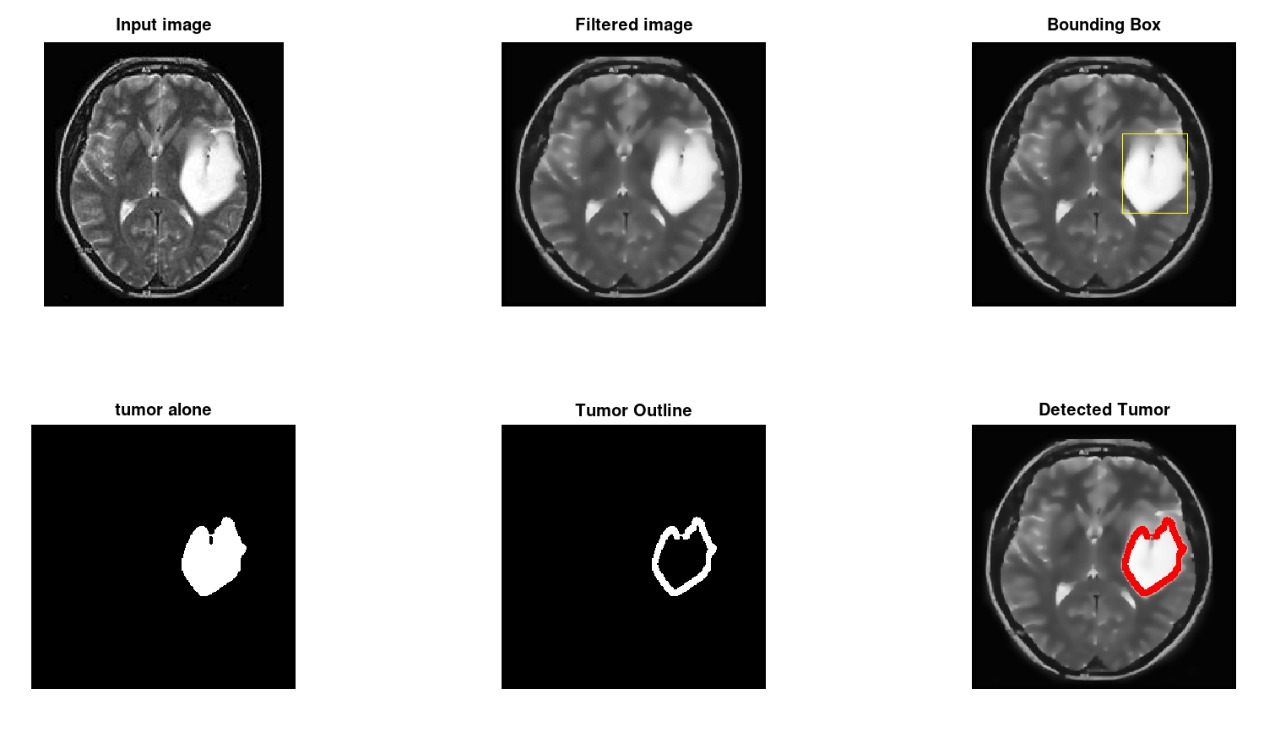
\includegraphics[width=105mm,height=65mm]{images/mri.jpeg}}
        \caption{Tumor segmentation}
        \label{fig:4}
    \end{figure}
\end{center}

\subsection{Classical Machine Learning}
\subsubsection{KNN based Methods}
\textbf{k-Nearest Neigbhours(KNN)} is a machine learning algorithm that looks at neighbouring pixels to determine the class of the current pixel.
Vrooman et.al. \cite{vrooman2007multi} automated KNN for segmentation. Conventional k-Nearest-Neighbor kNN classification, which has been successfully applied to classify brain tissue in MR data, requires training on manually labeled subjects. This manual labeling is a laborious and time-consuming procedure. In this work, a new fully automated brain tissue classification procedure is presented, in which kNN training is automated. This is achieved by non-rigidly registering the MR data with a tissue probability atlas to automatically select training samples, followed by a post-processing step to keep the most reliable samples. The accuracy of the new method was compared to rigid registration-based training and to conventional kNN-based segmentation using training on manually labeled subjects for segmenting gray matter (GM), white matter (WM) and cerebrospinal fluid CSF in 12 data sets. Furthermore, for all classification methods, the performance was assessed when varying the free parameters. Finally, the robustness of the fully automated procedure was evaluated on 59 subjects. The automated training method using non-rigid registration with a tissue probability atlas was significantly more accurate than rigid registration. For both automated training using non-rigid registration and for the manually trained kNN classifier, the difference with the manual labeling by observers was not significantly larger than inter-observer variability for all tissue types. From the robustness study, it was clear that, given an appropriate brain atlas and optimal parameters, our new fully automated, non-rigid registration-based method gives accurate and robust segmentation results. A similarity index was used for comparison with manually trained kNN. The similarity indices were 0.93, 0.92 and 0.92, for CSF, GM and WM, respectively. It can be concluded that our fully automated method using non-rigid registration may replace manual segmentation, and thus that automated brain tissue segmentation without laborious manual training is feasible.

\textbf{KNN with Tissue Type Bias}: This was proposed in Steenwijk et.al. \cite{steenwijk2013accurate}. The segmentation and volumetric quantification of white matter (WM) lesions play an important role in monitoring and studying neurological diseases such as multiple sclerosis (MS) or cerebrovascular disease. This is often interactively done using 2D magnetic resonance images. Recent developments in acquisition techniques allow for 3D imaging with much thinner sections, but the large number of images per subject makes manual lesion outlining infeasible. This warrants the need for a reliable automated approach. Here the authors aimed to improve k nearest neighbor (kNN) classification of WM lesions by optimizing intensity normalization and using spatial tissue type priors TTPs.
The kNN-TTP method used kNN classification with 3.0 T 3DFLAIR and 3DT1 intensities as well as MNI-normalized spatial coordinates as features. Additionally, TTPs were computed by nonlinear registration of data from healthy controls. Intensity features were normalized using variance scaling, robust range normalization or histogram matching. The algorithm was then trained and evaluated using a leave-one-out experiment among 20 patients with MS against a reference segmentation that was created completely manually. The performance of each normalization method was evaluated both with and without TTPs in the feature set.Volumetric agreement was evaluated using intra-class coefficient (ICC), and voxelwise spatial agreement was evaluated using Dice similarity index (SI). Finally, the robustness of the method across different scanners and patient populations was evaluated using an independent sample of elderly subjects with hypertension. 

KNNs have also been administered for brain tumor segmentation. Havaei et.al. \cite{havaei2014efficient} used KNN for an interactive tumor segmenation. This  task  is most  frequently  tackled  using  machine  learning methods that generalize across brains, by learning from training brain imagesin order to generalize to novel test brains. However this approachfaces many obstacles that threaten its performance, such as theability to properly perform multi-brain registration or brain-atlasalignment,  or  to  extract  appropriate  high-dimensional  featuresthat support good generalization. These operations are both non-trivial  and  time-consuming,  limiting  the  practicality  of  theseapproaches in a clinical context. In this paper, the authors propose to sidestep these issues by approaching the problem as one ofwithin braingeneralization. Specifically, they propose a semi-automatic method that segments a given brain by training and generalizing within that  brain  only,  based on some minimum user interaction.They investigate how k nearest neighbors (kNN), arguably the simplestmachine learning method available, combined with the simplestfeature vector possible raw MR signal + (x,y,z) position can becombined into a method that is both simple, accurate and fast.Results  obtained  on  the  online  BRATS  dataset  reveal  that  our method is fast and second best in terms of the complete and core test set tumor segmentation. 
\newpage
\subsubsection{K Means Clustering Based Methods}
K Means Clustering unkike KNN is an unsupervised algorithm and clusters similar data points together. Medical image segmentation using k-means clustering by Ng et.al. \cite{ng2006medical} leverages this unsupervised algorithm to cluster similar images together. They proposed a methodology that incorporates k-means and improved watershed segmentation algorithm for medical image segmentation. The use of the conventional watershed algorithm for medical image analysis is widespread because of its advantages, such as always being able to produce  a  complete    division    of    the    image.    However,    its    drawbacks  include  over-segmentation  and  sensitivity  to   false   edges.   The authors  address   the   drawbacks   of   the   conventional watershed algorithm when it is applied to medical   images   by   using   K-means   clustering   to   produce  a  primary  segmentation  of  the  image  before  they   appied their   improved   watershed   segmentation   algorithm   to   it.   The   K-means   clustering   is   an   unsupervised  learning  algorithm,  while  the  improved  watershed   segmentation   algorithm   makes   use   of automated  thresholding  on  the  gradient  magnitude  map  and  post-segmentation  merging  on  the  initial  partitions  to  reduce  the  number  of  false  edges  and  over-segmentation.   By   comparing   the   number   of   partitions  in  the  segmentation  maps  of  50  images,  we  showed   that   our   proposed   methodology   produced   segmentation  maps  which  have  92\%  fewer  partitions  than    the    segmentation    maps    produced    by the conventional watershed algorithm. The results are as seen in Fig \ref{fig:5}.

\begin{center}
    \begin{figure}[!h!t!b]
        \centerline{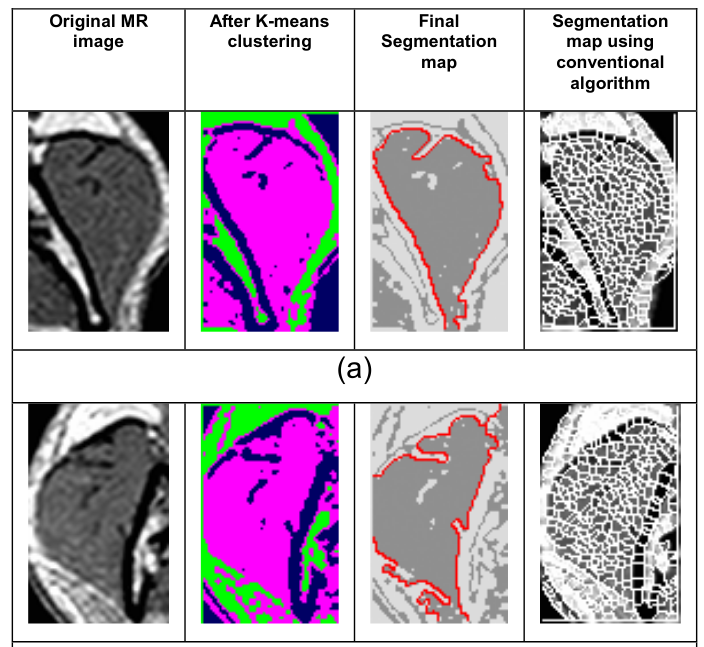
\includegraphics[width=105mm,height=95mm]{images/k-means.png}}
        \caption{Segmentation using k means clustering} 
        \label{fig:5}
    \end{figure}
\end{center}

Dhanachandra et.al. \cite{dhanachandra2015image} used K-means and sustractive clustering together to achieve segmentation. Image segmentation is the classification of an image into different groups. Many researches have been done in the area of image segmentation using clustering. There are different methods and one of the most popular methods is k-means clustering algorithm.K -means clustering algorithm is an unsupervised algorithm and it is used to segment the interest area from the background. But before applying K-means algorithm, first partial stretching enhancement is applied to the image to improve the quality of theimage. Subtractive clustering method is data clustering method where it generates the centroid based on the potential value of thedata points. So subtractive cluster is used to generate the initial centers and these centers are used in k-means algorithm for the segmentation of image. Then finally medial filter is applied to the segmented image to remove any unwanted region from the image. 
\newpage
\subsection{Deep Learning Methods}
While classical machine learning algorithms have been in several cases adequate for the task at hand, when it comes to segmenting compicated patterns, RGB images etc, Deep Learning far outclasses the methods discussed so far and defines the benchmarks for quality in the current world of technology. There are several methods out there. Let us review and discuss the most prominent ones.

\subsubsection{Conv Encoder-Decoder Architecture}
Long et.al. \cite{long2015fully} started the trend of using fully convolutional models for semantic segementation. This consisted of a convolutional encoder and a decoder.

\begin{center}
    \begin{figure}[!h!t!b]
        \centerline{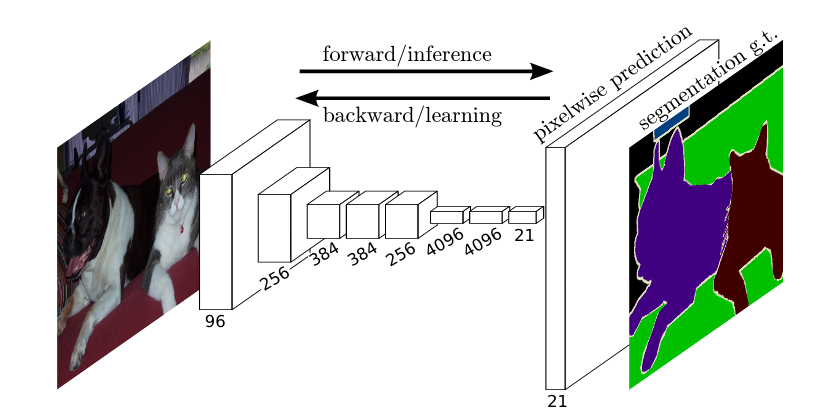
\includegraphics[width=135mm,height=85mm]{images/encdec.png}}
        \caption{An encoder decoder based architecture where a constricting encoder reduces the image to a latent space $z$ and a decoder extracts a segmentation map from this feature space. The feature space effectively contains the data of all pattens and characteristics of the image. Effective construction of this is the key to such models}
        \label{fig:8}
    \end{figure}
\end{center}
Convolutional networks are powerful visual models that yield  hierarchies  of  features. The authors demonstrated that  convolutional networks by themselves, trained end-to-end, pixels-to-pixels,  exceeded  the  state-of-the-art  in  semantic  segmentation at that time.Their key insight was  to  build  “fully  convolutional” networks  that  take  input  of  arbitrary  size  and  produce correspondingly sized  output  with  efficient  inference  andlearning.  They defined and detailed the space of fully convolutional networks, explained their application to spatially denseprediction tasks, and drew connections to prior models. 
\newpage
Their models also combined data from high and low resolution space as seen in \ref{fig:9} and this enabled them to prevent to learn a multi-resolution analysis. Such an analysis without deep learning would have required complex transformations as simply taking a Discrete Wavelet Transform might not be suitable for the task given at hand. 


\begin{center}
    \begin{figure}[!h!t!b]
        \centerline{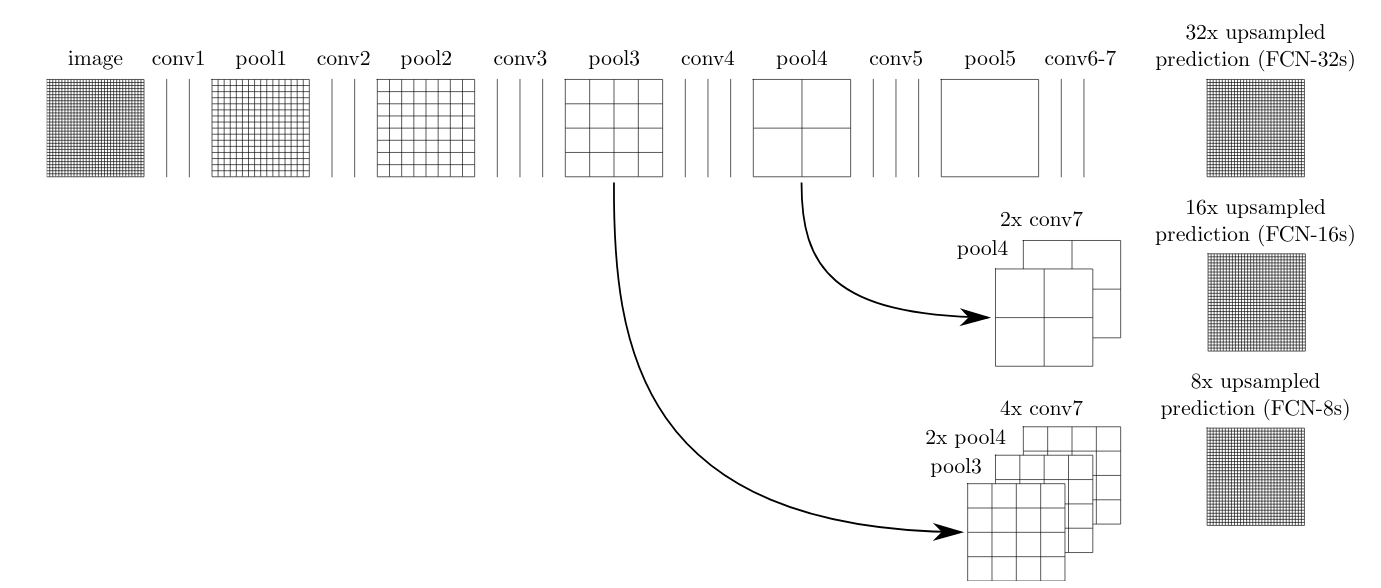
\includegraphics[width=175mm,height=95mm]{images/fcn.png}}
        \caption{"Multi resolution encoding in the feature space"}
        \label{fig:9}
    \end{figure}
\end{center}

 This simple model may be trained in 2 different ways. It could be trained end-to-end where the where all the layers are trainable at once. Alternatively, such a model could be trained in a stacked manner where each layer in depth is added and trained with the corresponding symmetric decoder and we iteratively add one layer after another till we reach our desired depth. 
\newpage 

\subsubsection{U-Nets}

U-net has been the go-to choice for semantic segmentation for medical images. Ronneberger et.al. \cite{ronneberger2015u} proposed this structure in 2015 with primary focus on medical image segmentation.Before reviewing the architecture, let us have a look at the general structure of the model in Fig. \ref{fig:6}. The U-Structure is a result of the symmetric contraction and expansion. As we propagate into the depth of any CNN, our field of vision on the input image increases but we may lose localization features and here comes the significance of passing the features from lower depth layers while upsampling for the output. At corner points or boundary regions, we may mirror parts of the input image so as to pass a consistent context. 
\begin{center}
    \begin{figure}[!h!t!b]
        \centerline{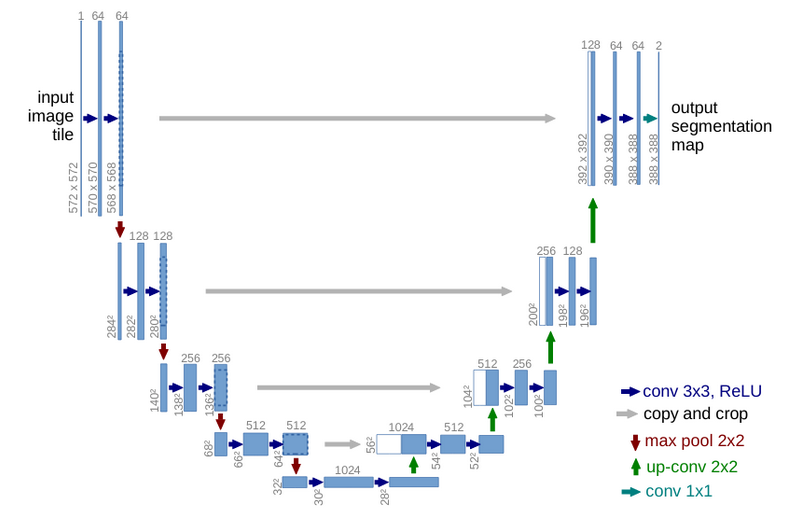
\includegraphics[width=135mm,height=115mm]{images/unet.png}}
        \caption{U-net architecture example for 32x32 pixels in the lowest resolution. Each bluebox corresponds to a multi-channel feature map. The number of channels is denotedon top of the box. The x-y-size is provided at the lower left edge of the box. Whiteboxes represent copied feature maps. The arrows denote the different operations.}
        \label{fig:6}
    \end{figure}
\end{center}

The Constricting part has repeated 3x3 conv - 2x2 maxPool units with number of feature channels doubling at each step. The ReLU activation layer is used. The expansive path has the upsampled featured map followed by 2x2 up-convolutions halving the number of feature channels at each step. The symmetrically opposite conv layer in the constricting block feeds its conv features to the corresponding block of the expansive path after upsampling which is followed by another convolution. Each block of convolution is defined as double convolution before pool as shown in Fig \ref{fig:6}.

The model is trained end to end as a supervised model with the input images and the corresponding segmentation maps. Use of large tiles as input is recommended so as to minimize the GPU overhead. This can be achieved by compromising the batch size. At the time of inference, batch size will be low but these large tiles will allow minimum execution time. A momentum-based optimizer like Adam may be used but the paper uses SDG with momentum 0.99 arguing that such a high momentum allows previous examples to further impact the current optimization step thereby taking a more general step in our optimization space. They used a softmax function followed by a cross entropy evaluation. 

The softmax function is as shown in eq \ref{softmax}

\begin{equation}
    \label{softmax}
        {p}_k(\vec{x}) = {\exp({a_k(\vec{x})}) \over \left(\sum_{k' =     1}^K \exp(a_{k'}(\vec{x}))\right)}
\end{equation}

where $a_k(\vec(x)$ is the activation of the last layer ie. the 1x1 Conv layer. This Softmax activation converts the ouput vector into probabilities and the elements of the obtained vector adds up to 1 along the dimension in which softmax is applied. Let us have a look at the cross entropy function as shown in the paper in eq. \ref{crossentropy} .
where $ \ell:\Omega \rightarrow {1,\dots,K} $ is the true label of each pixel and $ w:\Omega \rightarrow \mathbb{R} $  is a weight map that they introduced to give some pixels more importance in the training.

\begin{equation} 
    \label{crossentropy} 
        E = \sum_{\vec{x} \in \Omega} w(\vec{x}) \log({p}_{\ell(\vec{x})}(\vec{x}))  
\end{equation}

Let us try and understand why cross entropy was used in the first place. Any segmentation map, as seen in the cover picture has labels its pixels into one of a finite set of classes. For Eg, lets have a look at the following segmentation map in \ref{fig:7}.

\begin{center}
    \begin{figure}[!h!t!b]
        \centerline{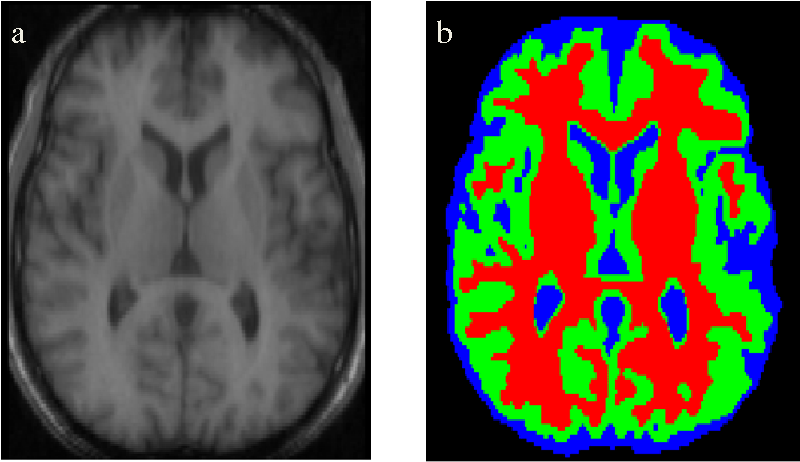
\includegraphics[width=95mm,height=75mm]{images/segmapunet.png}}
        \caption{A segmentation map using UNET. Note that each pixel in the given segmentation map is one of 3 classes of the 3 different colours}
        \label{fig:7}
    \end{figure}
\end{center}

As entropy is a quantification of the uncertainty in a system, the approach taken in the loss is a probabilistic one which aims to reduce the uncertainty in the class most probable for each pixel.It is maximum when all events are equiprobable and zero when one event is certain and the remaining are zero (In our case, the exact nature of the pixel is certain).There is an inherent need to give some pixels more importance than others in medical image analysis. For eg. Tumor cells may be more important to be correctly segmented than healthy cells as we definitely do not want to label a sick patient healthy. Additionally such a weight map must also deal with the class imbalances as the healthy cells are much more in number than the unhealthy ones. Lets have the formal definition of the weight map from the paper after evaluation of the seperation borders from morphological operations:

\begin{equation} 
    \label{weightmap}
    w(\vec{x}) = w_c(\vec{x}) + w_0 \cdot \exp\left( - \frac{(d_1(\vec{x}) + d_2(\vec{x}))^2}{2\sigma^2}\right ) 
\end{equation}

 where $w_c:\Omega \rightarrow \mathbb{R}$ is the weight map to balance the class frequencies, $d_1:\Omega \rightarrow \mathbb{R}$ denotes the distance to the border of the nearest cell and $d_2:\Omega \rightarrow \mathbb{R}$ the distance to the border of the second nearest cell. In their experiments they set $w_0 = 10$ and $ \sigma \approx 5 $ pixels.

 The weights of the architecture overall, are initialized as sampled from Gaussian Distributions with a standard deviation of $\sqrt{2/N}$, where $N$ denotes the number of incoming nodes of one neuron.

 \textbf{The $w_c$ concept is crucial as normally medical image datasets are unbalanced as healthy samples are usually greater than unhealthy samples. We must ensure that we weigh the unhealthy samples by a higher weight so as to not introduce a bias into the model towards healthy patients.}

 \subsubsection{Grad-CAM : Visual Explanations from Deep Networks via Gradient-based Localization}

 Selvaraju et.al. \cite{selvaraju2017grad} proposed a gradient based method that looks for patterns in the input image that force the activation of an output. These are known as Class Activation Maps. If we just have a dataset labelled healthy and unhealthy and we can get the Class Activation Map (CAM) of the data then we can get the input patterns that firce the activation of the unhealthy class and hence we can effectively "segment" the affected area.

 For a better understanding of the concept involved, we can refer to Fig \ref{fig:10}

\begin{center}
    \begin{figure}[!h!t!b]
        \centerline{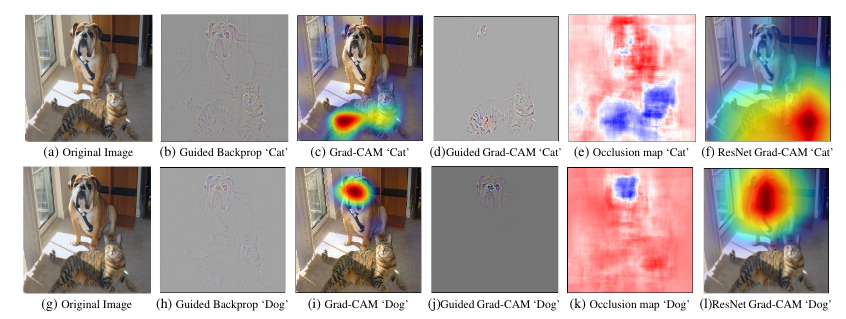
\includegraphics[width=175mm,height=75mm]{images/gradcampap.png}}
        \caption{Class Activation Maps achieved through this paper. Note the heatmap coressponds only to those regions which cause the class to be activated. Especially the ResNet GradCAM (Extreme Right)} 
        \label{fig:10}
    \end{figure}
\end{center}

This concept is generalizable to several tasks even other than image processing. However, since we are discussing everything with respect to localizing patterns causing the activation of the respective classes in medical images, our prime area of interest shall remain Computer Vision. that is the top most branch of Fig. \ref{fig:11}.GradCAMs rely on Global Average Pooling and their relationship and dependence is a matter of much interest as will be discussed later.
\newpage
\begin{center}
    \begin{figure}[!h!t!b]
        \centerline{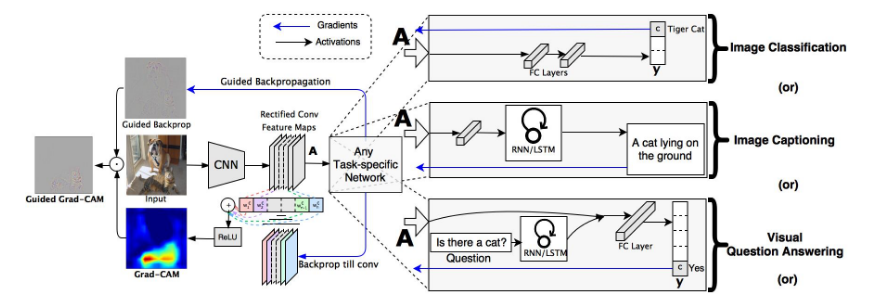
\includegraphics[width=175mm,height=85mm]{images/gradcamnet.png}} 
        \caption{The proposed methodology of achieving GradCAM}
        \label{fig:11}
    \end{figure}
\end{center}

A decent benchmark for performance evaluation would be the region of interest for a human to identify the said class from the image and the respective difference in the probablility distributions formed by evaluating the most probable region of attention paid by by the human as against the distribution suggested by the heatmap of the model.

It is noteworthy that this work using GradCAMs and Guided GradCAMs is revolutionary in the field of Computer Vision as in addition to the functions discussed these also refer to the regions in the input image the output is most vulnerable to thereby indicating the region of the input which, if attacked by certain amount of noise would cause misclassification. This inspired Protective Networks and Attacks on Vision models leading to a whole new branch of research.

\newpage
\section{Proposed Methodology}

\subsubsection{The Problem Statement}
The problem statement taken under consideration is the kaggle challenge hosted by KAGGLE named : \textbf{"Histopathologic Cancer Detection"} which aims to \textbf{ Identify metastatic tissue in histopathologic scans of lymph node sections.} 
\subsubsection{Dataset}

The dataset is as follows :

\textbf{220k training images and 57k evaluation images}. The dataset is a subset of the PCam dataset and the only difference between these two is that all duplicate images have been removed. The PCam dataset is derived from the Camelyon16 Challenge dataset which contains 400 H\&E stained whole slide images of sentinel lymph node sections that were acquired and digitized at 2 different centers using a 40x objective. The PCam's dataset including this one uses 10x undersampling to increase the field of view, which gives the resultant pixel resolution of 2.43 microns.

According to the data description, there is a 50/50 balance between positive and negative examples in the training and test splits. However, the training distribution seems to be 60/40 negatives/positives)(. A positive label means that there is at least one pixel of tumor tissue in the center region (32 x 32px) of the image. Tumor tissue in the outer region of the patch does not influence the label. This means that a negatively labeled image could contain metastases in the outer region. Thus, it would be a good idea to crop the images to the center region.


This dataset is a combination of two independent datasets collected in Radboud University Medical Center (Nijmegen, the Netherlands), and the University Medical Center Utrecht (Utrecht, the Netherlands). The slides are produced by routine clinical practices and a trained pathologist would examine similar images for identifying metastases. However, some relevant information about the surroundings might be left out with these small-sized image samples.
Is it valid? Does it reflect our expectations?

According to the data description, the dataset has been stripped of duplicates. However, this has not been confirmed by testing.

    For the entire dataset, when the slide-level label was unclear during the inspection of the H\&E-stained slide, an additional WSI with a consecutive tissue section, immunohistochemically stained for cytokeratin, was used to confirm the classification.


\newpage
\section{Bibliography}
\bibliographystyle{unsrt}  
\bibliography{references}  


%%% Comment out this section when you \bibliography{references} is enabled.

\end{document}
